\section{Software Choice}
The hardware choice and implementation includes a software that can handle them. The software choice will be explained in this section, describing the use of the Kernel, and the principle of scheduling.

\subsection{Kernel}
The chosen kernel allows to control the tasks and then the behavior of the vehicle through clocks, to have a precise and constant schedule. This propriety make possible to export it on another kind of processor and still have the same render, as long as it have a frequency high enough to process all the data needed.\\
The Kernel advantage is also the definition of semaphores, priorities, and critical regions, that the system will use to choose which task to run, and how often it should be. This Kernel allows also to program in Arduino language which is C++, and can run C code, with the use of different files.



\subsection{Scheduling}\label{sec:scheduling}
For running the code on the arduino PCB, and be able to manage all the sensors at the same time, a scheduling is needed. Indeed, the PCB must be able to recieve and process the data from the GoT system, the hall sensors, the magnetometer and the X-bee to make a decision related to the planned route to follow. This decision must affect at the same time the speed through the motor, and the steering through the servo.
A description of the scheduling principle and its function will be described.


\subsubsection{Semaphores}
In programming, a semaphore is a variable or abstract data that is used to prioritize the different tasks to use. It allows a multiprogramming, with functions that use different ressources and time, and does not interact with each others direcly. Running them independently ease the indent of the code.


\subsubsection{Tasks}
The different functions of the vehicle have been separated into multiple tasks, that can switch regarding to their priority. Five tasks are created to control the vehicle:

\begin{lstlisting} [caption = {Implementation of the tasks}, label = {lst:tasks}]

  task1 = k_crt_task(tSpeed, 10, stack, 300);         	   // Hall Sensors
  task2 = k_crt_task(SpeedControl, 12, stack2, 300); 	   // Speed control
  task3 = k_crt_task(GoT,14,stack5,1000);        		   // GoT and protocol handling
  task4 = k_crt_task(LeadCompensator, 13, stack4, 300);    // Distance Control
  task5 = k_crt_task(SteeringControl, 11, stack3, 1000);   // Angular control

\end{lstlisting}

Those declarations of the tasks are made thanks to the function k\_crt\_task needing the name of the function to run, it's priority, the area to use and it's lenght. The implementation of this function can be seen below.


\begin{lstlisting} [caption = {Declaration of the tasks}, label = {lst:tasks}]
 struct k_t *k_crt_task (void (*pTask) (void), char prio, char *pStk, int stkSize);
 
\end{lstlisting}


\textbf{Hall Sensors:}
The two hall sensors of the two belts are read at a certain frequency, and knowing the distance the vehicle moves during a full turn of the drive wheel, the real speed can be calculated independently from each other belts.\\
When the belts are not running the maximum time to run the task is 5.63µs, and when the belts are running it's 8.39µs.
The maximum speed of vehicle is 3 $m \cdot s^{-1}$, and a turn of the gear wheel is 166mm. To get a pulse every full turn of the gear wheel at the highest speed, the sampling period has to be $\frac{0.166}{3}={55.3ms}$, and for a quarter of turn it should be 4 time less so every 14ms. On another side, the sampling time of reading the magnetometer has to be 2 times less the highest frequency sampling of the system, but to be secure, the sampling time is chosen at 3.5 times less, giving a minimum period of 4ms period.

\textbf{Speed Control:}
A wanted speed value is compared to the actual speed, and the resulting error is the input of the Velocity PI-Controller, that will set a new speed according to the reference.\\
The running time of this task is 386µs. For a precise control of the speed a half of the period of the hall sensor is chosen, the minimum period will be 2ms.


\textbf{GoT System and Communication Protocol:}
This task is the communication protocol handling, that receives on the vehicle the position that the GoT system sended. It will receive data from the computer, and convert it into a position so that the distance control can calculate the new heading to follow.\\
The running time of the GoT System and Communication Protocol task is 395µs, and the sampling time of the GoT system giving a new position is 100ms.

\textbf{Distance control:}
If the angular control is in charge of the direction wanted, it can not control the position from the line wanted to be on. The task Distance Control calculate the distance of the vehicle from the line it should follow, and calculate a new heading for the angular control to follow to get back on the line. This is the outer loop from the Steering Model, seen in \secref{sec:SteeringModel}.\\
The running time of the Distance Control is 153.6µs, and it runs just after the GoT System and Communication Protocol, so has a sampling time of also 100ms.

\textbf{Angular Control:}
The steering task gets the reading from the magnetometer, and transform them in the coordinate system that fits the model. Then those values are converted into a heading angle, that will be used in the steering P-Controller to calculate the new angle to follow from the angle wanted. The decision will be sent directly to the servo. This is the inner loop from the Steering Model, seen in \secref{sec:SteeringModel}.\\
The running time of the Angluar Control is the largest one with 1.7ms needed to send a new angle. However, the minimum time to send a new angle to the servo is 30ms because of the sampling time of the servo. The period of this task has then to be 30ms.\\\\


A recapitulation of the parameters can be seen on \tableref{scheduleParameters}.

\begin{table} [H]
	\begin{tabular}{|l|l|l|l|l|l|}
								
\hline
\textbf{n°}  & \textbf{Task}   	 & \textbf{Priority}	& \textbf{Max. Time to Run} 	& \textbf{Min. Period} & \textbf{CPU Used}\\
\hline
1			 &	Hall Sensors	 & 2				&	\si{8,39 \mu s}			    &	\si{4 ms}			  & 0,2\%	  \\
\hline
2			 &	Speed Control	 & 3				&	\si{386\ \mu s}				&	\si{2 ms}			  &	19,3 \%   \\
\hline
3			 &	GoT and Protocol & 4				&	\si{395 \mu s}			    &	\si{100 ms}			  &	0,395 \%  \\
\hline
4			 &	Distance Control & 4				&	\si{153,6 \mu s} 			&	\si{100 ms} 	  	  &	0,154 \%  \\
\hline
5			 &	Angular Control	 & 1				&	\si{1,7  ms}			    &	\si{30 ms}			  &	5,7 \%    \\
\hline		
	\end{tabular}
	\caption{Calculations of the steering parameters.}	
	\label{scheduleParameters}						
\end{table}	

In the \tableref{scheduleParameters}, the Maximum Time to Run is the time the task needs to complete a full turn of the loop. The Minimum Period is the sampling time for the task, to run every time period. The CPU used is the percentage used by the task of the CPU, which is the ratio between the Maximum Time to Run and the Minimum Period.

\subsubsection{Queue}
The tasks are meant to be done at the time they are told to be done, ensuring the good control of the vehicle. But some functionnalities are not critical, and can wait until the processor have time to do them.\\
When a task is running and another one with a higher priority do a request to run, the actual task will be sotred and wait until the higher one will be done. The order of the task will be done regarding to their priorities.


\subsubsection{Request and Priorities}
The tasks ask a request of running every period of time regarding their respective setup, the global view of these request can be seen in \figref{scheduleRequest}.

 \begin{figure}[H]
	\centering
	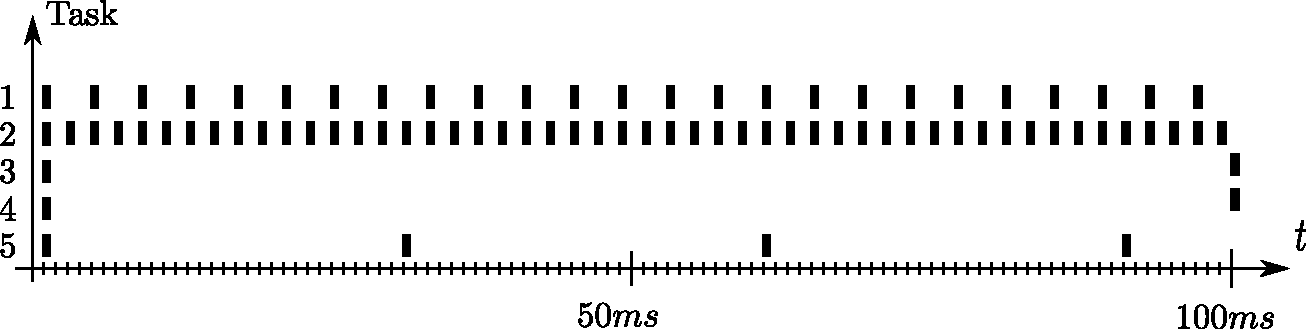
\includegraphics[scale=0.6]{figures/scheduleRequest.pdf}
	\caption{An overview of the tasks request during 100ms, the larger period task possible.}
	\label{scheduleRequestd}
\end{figure}


When two task are requesting at the same time to run, the order is chosen regarding to the priorities, that is set at the initialisation. The task are ran when they ask it, but interrupted when a higher priority task is asking to run, and will finish when all the higher priorities will be done. An example of this case can be seen in \figref{schedulePriorities}.\\
The priorities of the task have been made to give the system the best stability. In this case, The angular sensor has the highest priority because it has a large period and running time, but is critical to the steering of the vehicle which is the main objective of this project. Then comes the hall sensors that is very fast to execute, and then the speed control which is so fast that is not critical to have it at a high priority. The last one is the GoT system and communication protocol along with the distance control, because of two things: first because it may enter in an infinite loop and block the system, and second and most of all because the main point of this project is to be able to run without the GoT system if something happend and block the communication.

 \begin{figure}[H]
	\centering
	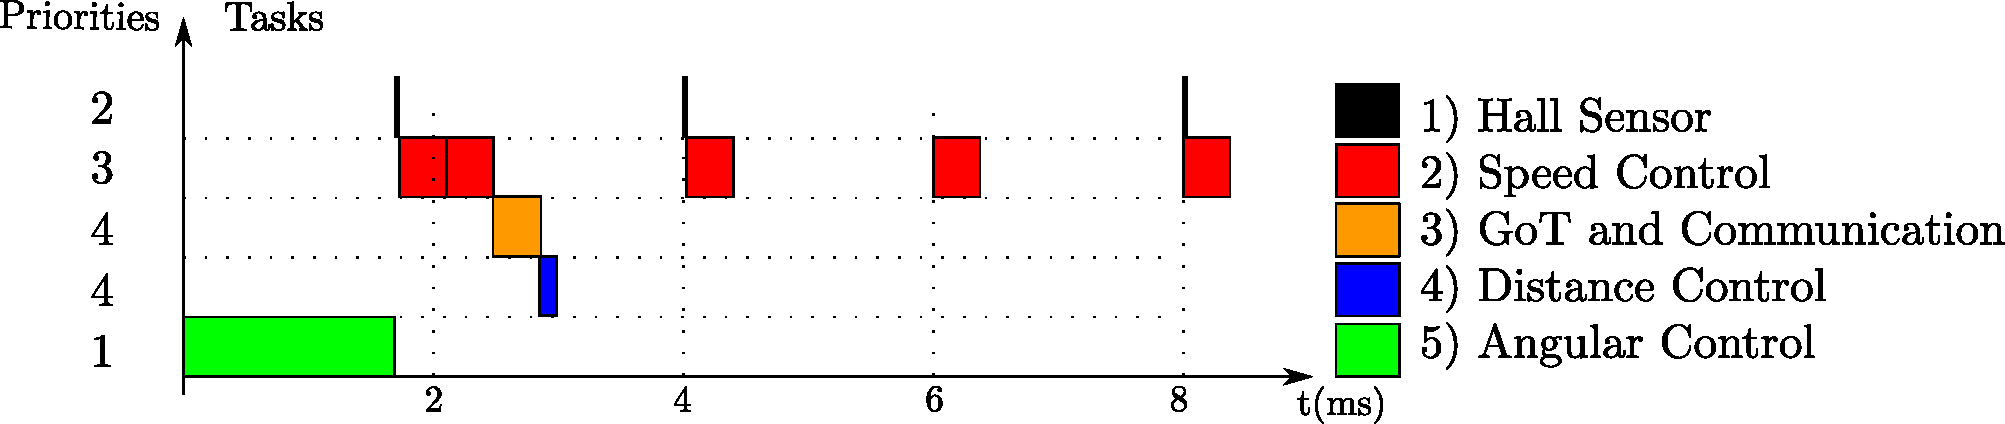
\includegraphics[scale=0.5]{figures/schedulePriorities.pdf}
	\caption{Schedule of the tasks at the starting time, regarding the priorities.}
	\label{schedulePriorities}
\end{figure}

As seen on the  \figref{schedulePriorities}, the angular control has the highest priority so it will run first, and the others will be registrered in a queue in order of priority. Then the hall sensors are second, and speed control after that. When the speed control will be running, it can do a second request to run because of it's sampling time. It will then run a second time just after that because it's priority is higher than the lasts tasks. The GoT and comunication will run after them, and in the end the Distance Control.\\
After a certain time, the task are stabilized, until the tasks with a large period are asked again.\\\\



Now that the harware and software choice have been described and explained, the sensors can be implemented, independently from each other.